\chapter{Resultados e Validação} \label{ch:results}

Com o simulador finalizado, é necessária a avaliação de seus resultados para que a implementação seja validada. A apresentação e a análise de simulações são feitas neste capítulo. Com o fim de se fazer a validação numérica, os resultados são comparados com soluções analíticas ou qualitativamente avaliados.

\alert{Talvez explicar melhor o objetivo deste capítulo}
\alert{Fazer um breve resumo das simulações executadas}
\alert{As simulações foram executadas em um computador com épsilon de máquina igual a \(2,2204460492503131e-16\)}

\section{Lançamento Oblíquo}

O lançamento oblíquo é um dos problemas clássicos de física básica. Considera-se uma partícula de massa \(\mass\) sujeita unicamente à ação de um campo gravitacional constante cuja aceleração da gravidade é \(\gravity\). Nessas condições, as equações de movimento para a partícula se tornam, simplesmente,
\begin{gather}
	\acceleration = \gravity, \label{eq:free_fall_translation}\\
	\angularAcceleration = \nullVector \label{eq:free_fall_rotation}.
\end{gather}

O instante inicial da simulação é definido como \(\initial{t}=0\), e o instante final é um valor arbitrário \(\final{t}\). A posição, a velocidade e a velocidade angular da partícula no instante inicial assumem, respectivamente, os valores \(\initial{\position}\), \(\initial{\velocity}\) e \(\initial{\angularVelocity}\). As equações \eqref{eq:free_fall_translation} e \eqref{eq:free_fall_translation} podem ser resolvidas por integração simples:
\begin{gather*}
	\acceleration\pqty{t} = \gravity, \\
	\velocity\pqty{t} = \initial{\velocity} + \int_{0}^{t} \acceleration\pqty{\tau} \dd{\tau} = \initial{\velocity} + \gravity\cdot t, \\
	\position\pqty{t} = \initial{\position} + \int_{0}^{t} \velocity\pqty{\tau} \dd{\tau} = \initial{\position} + \initial{\velocity}\cdot t + \gravity\cdot \dfrac{t^2}{2}, \\
	\angularVelocity\pqty{t} = \initial{\angularVelocity} + \int_{0}^{t} \nullVector \dd{\tau} = \initial{\angularVelocity}.
\end{gather*}

Por simplicidade, considera-se que o movimento ocorra apenas no plano \(\xAxis\yAxis\), que a gravidade atue no sentido negativo do eixo \(\yAxis\), isto é, \(\gravity = -\gravityScalar\cdot\yUnit\) com \(\gravityScalar>0\), e que a partícula não possua rotação, como representado na figura \ref{fig:free_fall}. Nessa situação, a posição em \(\yAxis\) da partícula também é chamada de altura.

\begin{figure}[h]
	\caption{O problema do lançamento oblíquo}
	% \vspace{-0.5cm}
	\begin{center}
		\alert{Colocar imagem representando o problema do lançamento oblíquo}
		% 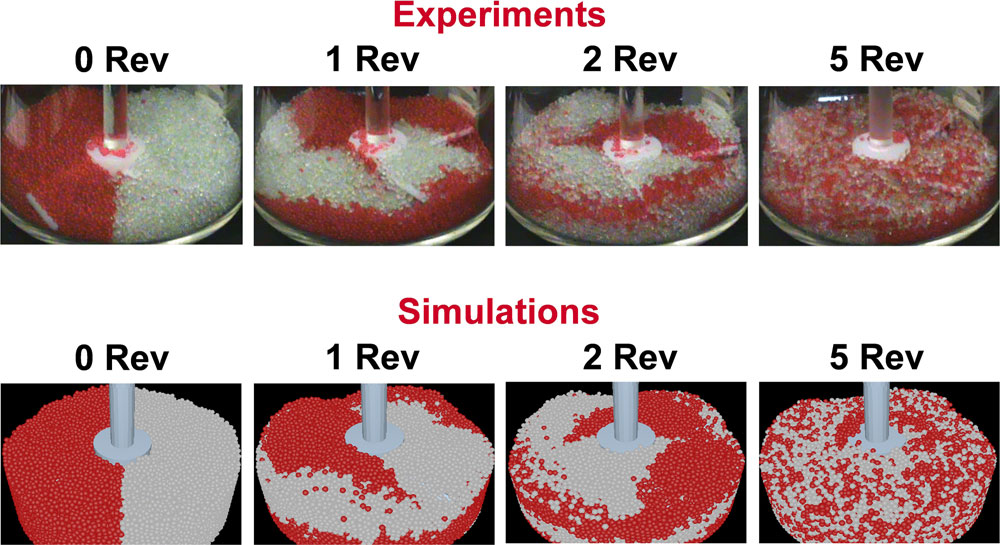
\includegraphics[width=0.65\textwidth]{images/drug_production.png}
	\end{center}
	% {\centerline{\includegraphics[scale=#2]{#1}}}
	% \vspace{-0.2cm}
	\label{fig:free_fall}
	\legend{Fonte: \alert{Citar fonte}.}
	% \vspace{-1cm}
\end{figure}

Com isso, escrevendo \(\position = \explicitVectorCoordinates{\positionScalar}\), \(\velocity = \explicitVectorCoordinates{\velocityScalar}\) e \(\acceleration = \explicitVectorCoordinates{\accelerationScalar}\), é obtida a solução como apresentada na tabela \ref{table:free_fall_solution}.

\begin{table}[h]
	\caption{Solução do problema do lançamento oblíquo}
	\label{table:free_fall_solution}

	\begin{equation*}
		% \arraycolsep=1.4pt
		\def\arraystretch{1.5}
		\begin{array}{lccc}
	\hline
		& \text{Direção } \xAxis 
		& \text{Direção } \yAxis 
		& \text{Direção } \zAxis
		\\
	\text{Posição} 
		& \positionx = \initial{\positionx} + \initial{\velocityx}\cdot \Dt
		& \positiony = \initial{\positiony} + \initial{\velocityy}\cdot \Dt - \dfrac{\gravityScalar\Dt^2}{2}
		& \positionz = \initial{\positionz} \\
	\text{Velocidade} 
		& \velocityx = \initial{\velocityx}
		& \velocityy = \initial{\velocityy} - \gravityScalar\cdot \Dt
		& \velocityz = 0 \\
	\text{Aceleração} 
		& \accelerationx = 0
		& \accelerationy = - \gravityScalar
		& \accelerationz = 0 \\
	\hline	
		\end{array}
	\end{equation*}
	\legend{Fonte: do Autor}
\end{table}

Embora seja um problema conceitualmente simples e de fácil resolução, o problema do lançamento oblíquo permite:
\begin{itemize}
\item A validação numérica da implementação do algoritmo de Gear em simulações sem colisões, mas com a atuação de forças de campo.
\item A análise da evolução do erro em função do passo de tempo.
\item A obtenção da evolução do erro com o tempo de simulação.
\end{itemize}



\alert{Mostrar o quanto o erro evolui com o aumento do tempo final de simulação}

\subsection{Estudo de Caso} \alert{Que título horrível!}

A fim de se compararem os resultados numéricos com a solução analítica, foram arbitrados os seguintes valores aos parâmetros do problema:
\begin{description}
	\item[Massa da partícula: ] \(\mass = 1\,\si\kilogram\);
	\item[Raio da partícula: ] \(\radius = 3\,\si\centi\metre\);
	\item[Posição inicial: ] \(\explicitVector{\initial{\positionx}}{\initial{\positiony}}{\initial{\positionz}} = \explicitVector{0}{0}{0}\si{\metre}\);
	\item[Velocidade inicial: ] \(\explicitVector{\initial{\velocityx}}{\initial{\velocityy}}{\initial{\velocityz}} = \explicitVector{10}{5}{0}\si[per-mode=symbol]{\metre\per\second}\);
	\alert{Confusão entre 10,5 e 10, 5 ??}
	\item[Aceleração inicial: ] \(\explicitVector{\initial{\accelerationx}}{\initial{\accelerationy}}{\initial{\accelerationz}} = \explicitVector{0}{0}{0}\si[per-mode=symbol]{\metre\per\square\second}\);
	\item[Instante final: ] \(\final{t} = 2\,\si\second\) 
	\item[Ordem de extrapolação: ] \(\taylorOrder = 7\)
	\item[Gravidade: ] \(\gravityScalar = 9,81\,\si[per-mode=symbol]{\metre\per\square\second}\)
	\item[Passo de tempo: ] \(\Dt = 10^{-3}\,\si\second\)
\end{description}
\alert{Usar uma tabela?}

Muito embora se trate de um problema bidimensional sem rotação, o simulador utiliza a formulação tridimensional e considera a evolução da velocidade angular da partícula.

Com esses parâmetros, foi calculada a trajetória da partícula através do simulador e da solução analítica como expostos na figura \ref{fig:falling_sphere}. O erro em função do tempo, por sua vez, é apresentado na figura \ref{fig:falling_sphere_error}

\begin{figure}[h]
	\caption{Solução do problema de lançamento oblíquo}
	% \vspace{-0.5cm}
	\begin{center}
		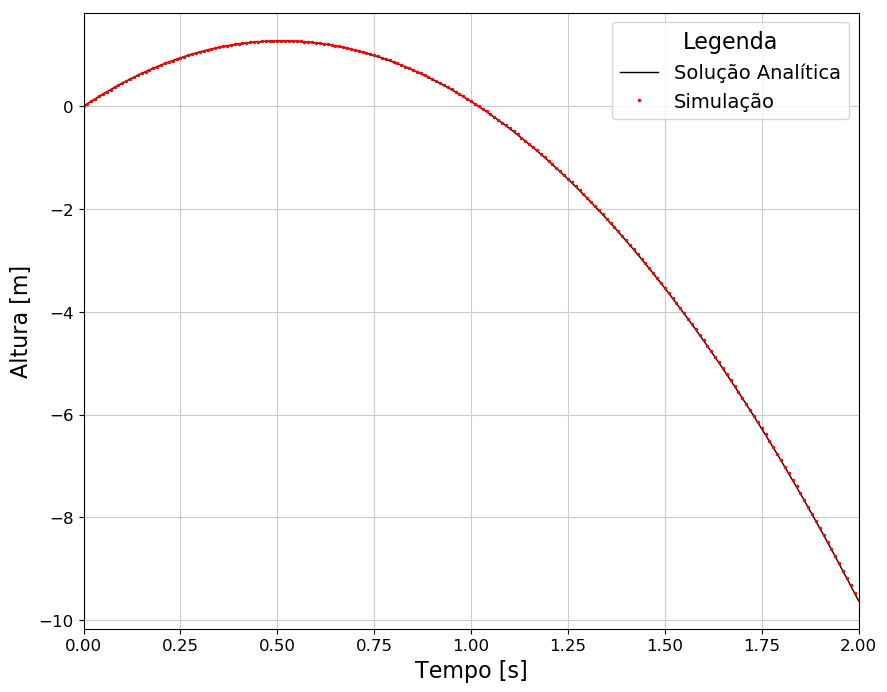
\includegraphics[width=0.8\textwidth]{images/falling_sphere/y_position.png}
	\end{center}
	% {\centerline{\includegraphics[scale=#2]{#1}}}
	% \vspace{-0.2cm}
	\label{fig:falling_sphere}
	\legend{Fonte: do Autor.}
	% \vspace{-1cm}
\end{figure}

\begin{figure}[h]
	\caption{Erro da solução do problema de lançamento oblíquo}
	% \vspace{-0.5cm}
	\begin{center}
		\alert{Inserir figura}
		% 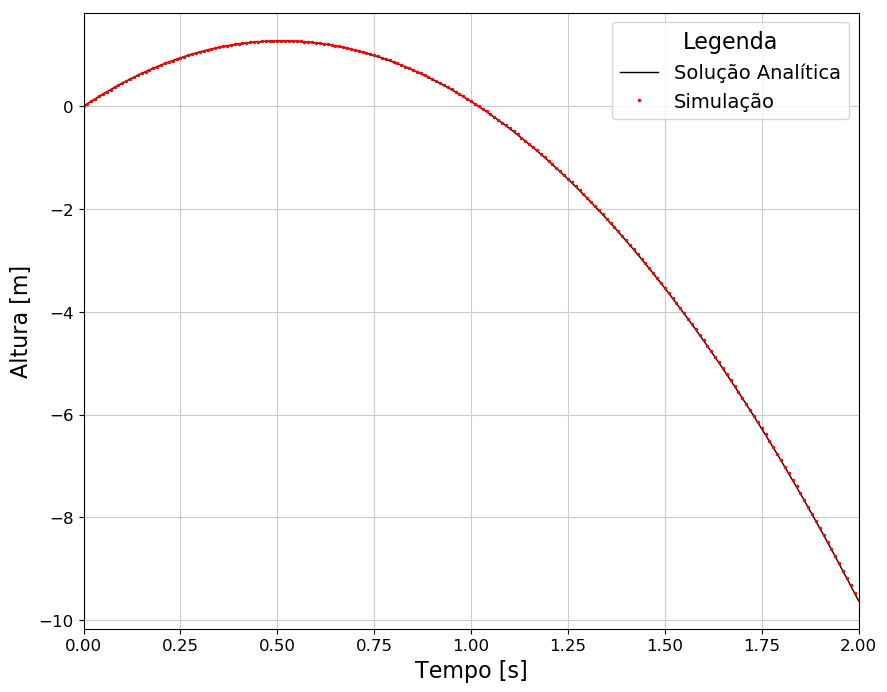
\includegraphics[width=0.8\textwidth]{images/falling_sphere/y_position.png}
	\end{center}
	% {\centerline{\includegraphics[scale=#2]{#1}}}
	% \vspace{-0.2cm}
	\label{fig:falling_sphere_error}
	\legend{Fonte: do Autor.}
	% \vspace{-1cm}
\end{figure}

\alert{Definir erro máximo}

\alert{Incluir arquivo .json em um apêndice para mostrar como a simulação é configurada?}

\subsection{Influência da Ordem de Extrapolação}

\subsection{Influência do Passo de Tempo}